All code we used to develop, train, and evaluate our models is available in Tensor2Tensor \citep{tensor2tensor}.
% \url{https://github.com/tensorflow/tensor2tensor}.

For all experiments we optimize with Adam~\citep{kingma2014adam}, and vary the learning rate as specified in~\cite{aiayn}. We train our models on both p100 and k40 GPUs, with batch sizes ranging from $1$ to $8$ per GPU.

\begin{table}[t]
\centering

\begin{tabular}{@{\hspace{.05cm}}c@{\hspace{.05cm}}c@{\hspace{.05cm}}c@{\hspace{.05cm}}c@{\hspace{.05cm}}c@{\hspace{.3cm}}c@{\hspace{.05cm}}c@{\hspace{.05cm}}c@{\hspace{.05cm}}c@{\hspace{.05cm}}c} \\ 
% Input & Bicubic & \regression & $\tau=1.0$ & $\tau=0.9$ & $\tau=0.8$ & Truth & \NN{} & GAN~\cite{srez} & GAN~\cite{srez} \\ 
% \endhead 
  {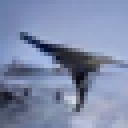
\includegraphics[width=.09\linewidth]{cifar10_303_cond_images/0/labeloutputs_cifar10_perp_2097_1070.png}} 
 & {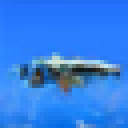
\includegraphics[width=.09\linewidth]{cifar10_303_cond_images/0/labeloutputs_cifar10_perp_2097_807.png}} 
 & {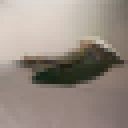
\includegraphics[width=.09\linewidth]{cifar10_303_cond_images/0/labeloutputs_cifar10_perp_2097_3910.png}} 
 & {
\includegraphics[width=.09\linewidth]{cifar10_303_cond_images/0/labeloutputs_cifar10_perp_2097_326.png}} 
 & {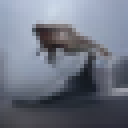
\includegraphics[width=.09\linewidth]{cifar10_303_cond_images/0/labeloutputs_cifar10_perp_2097_1255.png}}
&  {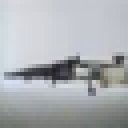
\includegraphics[width=.09\linewidth]{cifar10_299_cond_images/0/labeloutputs_cifar10_perp_2047_1069.png}}
& {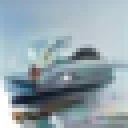
\includegraphics[width=.09\linewidth]{cifar10_299_cond_images/0/labeloutputs_cifar10_perp_2047_1213.png}}
& {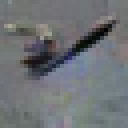
\includegraphics[width=.09\linewidth]{cifar10_299_cond_images/0/labeloutputs_cifar10_perp_2047_2077.png}}
& {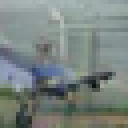
\includegraphics[width=.09\linewidth]{cifar10_299_cond_images/0/labeloutputs_cifar10_perp_2047_2222.png}}
& {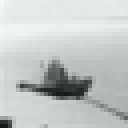
\includegraphics[width=.09\linewidth]{cifar10_299_cond_images/0/labeloutputs_cifar10_perp_2047_325.png}} 
 \\ [-0.75mm]
 {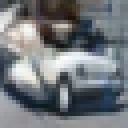
\includegraphics[width=.09\linewidth]{cifar10_303_cond_images/1/labeloutputs_cifar10_perp_2097_1755.png}} 
 & {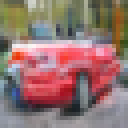
\includegraphics[width=.09\linewidth]{cifar10_303_cond_images/1/labeloutputs_cifar10_perp_2097_2368.png}} 
 & {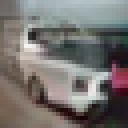
\includegraphics[width=.09\linewidth]{cifar10_303_cond_images/1/labeloutputs_cifar10_perp_2097_2580.png}} 
 & {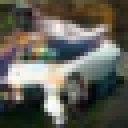
\includegraphics[width=.09\linewidth]{cifar10_303_cond_images/1/labeloutputs_cifar10_perp_2097_3094.png}} 
 & {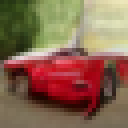
\includegraphics[width=.09\linewidth]{cifar10_303_cond_images/1/labeloutputs_cifar10_perp_2097_674.png}}
 & {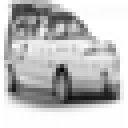
\includegraphics[width=.09\linewidth]{cifar10_299_cond_images/1/labeloutputs_cifar10_perp_2047_1331.png}}
& {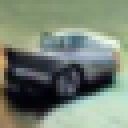
\includegraphics[width=.09\linewidth]{cifar10_299_cond_images/1/labeloutputs_cifar10_perp_2047_1754.png}}
& {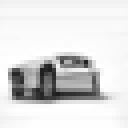
\includegraphics[width=.09\linewidth]{cifar10_299_cond_images/1/labeloutputs_cifar10_perp_2047_1849.png}}
& {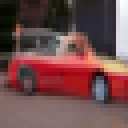
\includegraphics[width=.09\linewidth]{cifar10_299_cond_images/1/labeloutputs_cifar10_perp_2047_265.png}}
& {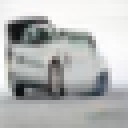
\includegraphics[width=.09\linewidth]{cifar10_299_cond_images/1/labeloutputs_cifar10_perp_2047_575.png}}
\\ [-0.75mm]
{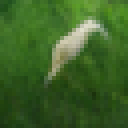
\includegraphics[width=.09\linewidth]{cifar10_303_cond_images/2/labeloutputs_cifar10_perp_2097_1072.png}}
& {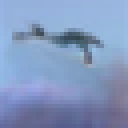
\includegraphics[width=.09\linewidth]{cifar10_303_cond_images/2/labeloutputs_cifar10_perp_2097_2191.png}}
& {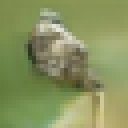
\includegraphics[width=.09\linewidth]{cifar10_303_cond_images/2/labeloutputs_cifar10_perp_2097_3050.png}}
& {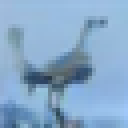
\includegraphics[width=.09\linewidth]{cifar10_303_cond_images/2/labeloutputs_cifar10_perp_2097_6.png}}
& {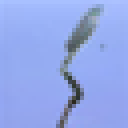
\includegraphics[width=.09\linewidth]{cifar10_303_cond_images/2/labeloutputs_cifar10_perp_2097_732.png}}
& {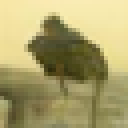
\includegraphics[width=.09\linewidth]{cifar10_299_cond_images/2/labeloutputs_cifar10_perp_2047_1391.png}}
& {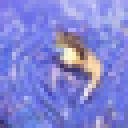
\includegraphics[width=.09\linewidth]{cifar10_299_cond_images/2/labeloutputs_cifar10_perp_2047_153.png}}
& {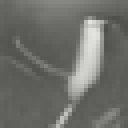
\includegraphics[width=.09\linewidth]{cifar10_299_cond_images/2/labeloutputs_cifar10_perp_2047_2188.png}}
& {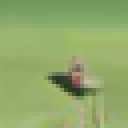
\includegraphics[width=.09\linewidth]{cifar10_299_cond_images/2/labeloutputs_cifar10_perp_2047_2298.png}}
& {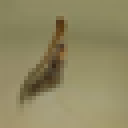
\includegraphics[width=.09\linewidth]{cifar10_299_cond_images/2/labeloutputs_cifar10_perp_2047_2303.png}}
\\  [-0.75mm]
{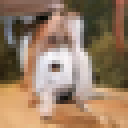
\includegraphics[width=.09\linewidth]{cifar10_303_cond_images/3/labeloutputs_cifar10_perp_2097_1003.png}}
& {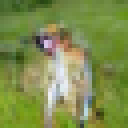
\includegraphics[width=.09\linewidth]{cifar10_303_cond_images/3/labeloutputs_cifar10_perp_2097_2362.png}}
& {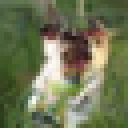
\includegraphics[width=.09\linewidth]{cifar10_303_cond_images/3/labeloutputs_cifar10_perp_2097_3040.png}}
& {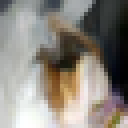
\includegraphics[width=.09\linewidth]{cifar10_303_cond_images/3/labeloutputs_cifar10_perp_2097_3257.png}}
& {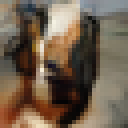
\includegraphics[width=.09\linewidth]{cifar10_303_cond_images/3/labeloutputs_cifar10_perp_2097_3610.png}}
&{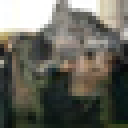
\includegraphics[width=.09\linewidth]{cifar10_299_cond_images/3/labeloutputs_cifar10_perp_2047_1647.png}}
& {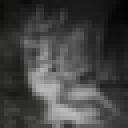
\includegraphics[width=.09\linewidth]{cifar10_299_cond_images/3/labeloutputs_cifar10_perp_2047_1672.png}}
& {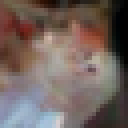
\includegraphics[width=.09\linewidth]{cifar10_299_cond_images/3/labeloutputs_cifar10_perp_2047_1673.png}}
& {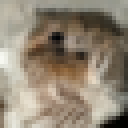
\includegraphics[width=.09\linewidth]{cifar10_299_cond_images/3/labeloutputs_cifar10_perp_2047_1987.png}}
& {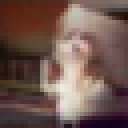
\includegraphics[width=.09\linewidth]{cifar10_299_cond_images/3/labeloutputs_cifar10_perp_2047_68.png}}
\\  [-0.75mm]
{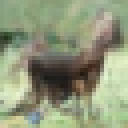
\includegraphics[width=.09\linewidth]{cifar10_303_cond_images/4/labeloutputs_cifar10_perp_2097_2756.png}}
& {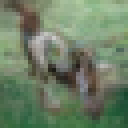
\includegraphics[width=.09\linewidth]{cifar10_303_cond_images/4/labeloutputs_cifar10_perp_2097_2859.png}}
& {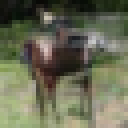
\includegraphics[width=.09\linewidth]{cifar10_303_cond_images/4/labeloutputs_cifar10_perp_2097_29.png}}
& {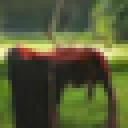
\includegraphics[width=.09\linewidth]{cifar10_303_cond_images/4/labeloutputs_cifar10_perp_2097_3963.png}}
& {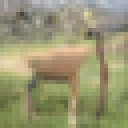
\includegraphics[width=.09\linewidth]{cifar10_303_cond_images/4/labeloutputs_cifar10_perp_2097_4086.png}}
& {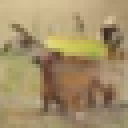
\includegraphics[width=.09\linewidth]{cifar10_299_cond_images/4/labeloutputs_cifar10_perp_2047_22.png}}
& {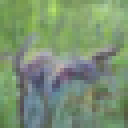
\includegraphics[width=.09\linewidth]{cifar10_299_cond_images/4/labeloutputs_cifar10_perp_2047_28.png}}
& {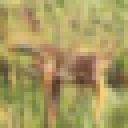
\includegraphics[width=.09\linewidth]{cifar10_299_cond_images/4/labeloutputs_cifar10_perp_2047_411.png}}
& {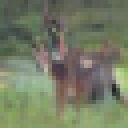
\includegraphics[width=.09\linewidth]{cifar10_299_cond_images/4/labeloutputs_cifar10_perp_2047_433.png}}
& {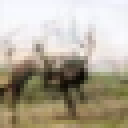
\includegraphics[width=.09\linewidth]{cifar10_299_cond_images/4/labeloutputs_cifar10_perp_2047_862.png}}
\\ [-0.75mm]
{\includegraphics[width=.09\linewidth]{cifar10_303_cond_images/5/labeloutputs_cifar10_perp_2097_1322.png}}
& {\includegraphics[width=.09\linewidth]{cifar10_303_cond_images/5/labeloutputs_cifar10_perp_2097_213.png}}
& {\includegraphics[width=.09\linewidth]{cifar10_303_cond_images/5/labeloutputs_cifar10_perp_2097_2233.png}}
& {\includegraphics[width=.09\linewidth]{cifar10_303_cond_images/5/labeloutputs_cifar10_perp_2097_4207.png}}
& {\includegraphics[width=.09\linewidth]{cifar10_303_cond_images/5/labeloutputs_cifar10_perp_2097_727.png}}
& {\includegraphics[width=.09\linewidth]{cifar10_299_cond_images/5/labeloutputs_cifar10_perp_2047_139.png}}
& {\includegraphics[width=.09\linewidth]{cifar10_299_cond_images/5/labeloutputs_cifar10_perp_2047_142.png}}
& {\includegraphics[width=.09\linewidth]{cifar10_299_cond_images/5/labeloutputs_cifar10_perp_2047_2453.png}}
& {\includegraphics[width=.09\linewidth]{cifar10_299_cond_images/5/labeloutputs_cifar10_perp_2047_2472.png}}
& {\includegraphics[width=.09\linewidth]{cifar10_299_cond_images/5/labeloutputs_cifar10_perp_2047_2572.png}}
\\ [-0.75mm]
{\includegraphics[width=.09\linewidth]{cifar10_303_cond_images/6/labeloutputs_cifar10_perp_2097_127.png}}
& {\includegraphics[width=.09\linewidth]{cifar10_303_cond_images/6/labeloutputs_cifar10_perp_2097_1907.png}}
& {\includegraphics[width=.09\linewidth]{cifar10_303_cond_images/6/labeloutputs_cifar10_perp_2097_2729.png}}
& {\includegraphics[width=.09\linewidth]{cifar10_303_cond_images/6/labeloutputs_cifar10_perp_2097_3895.png}}
& {\includegraphics[width=.09\linewidth]{cifar10_303_cond_images/6/labeloutputs_cifar10_perp_2097_4111.png}}
& {\includegraphics[width=.09\linewidth]{cifar10_299_cond_images/6/labeloutputs_cifar10_perp_2047_126.png}}
& {\includegraphics[width=.09\linewidth]{cifar10_299_cond_images/6/labeloutputs_cifar10_perp_2047_1431.png}}
& {\includegraphics[width=.09\linewidth]{cifar10_299_cond_images/6/labeloutputs_cifar10_perp_2047_2228.png}}
& {\includegraphics[width=.09\linewidth]{cifar10_299_cond_images/6/labeloutputs_cifar10_perp_2047_2543.png}}
& {\includegraphics[width=.09\linewidth]{cifar10_299_cond_images/6/labeloutputs_cifar10_perp_2047_719.png}}
\\ [-0.75mm]
{\includegraphics[width=.09\linewidth]{cifar10_303_cond_images/7/labeloutputs_cifar10_perp_2097_149.png}}
& {\includegraphics[width=.09\linewidth]{cifar10_303_cond_images/7/labeloutputs_cifar10_perp_2097_2604.png}}
& {\includegraphics[width=.09\linewidth]{cifar10_303_cond_images/7/labeloutputs_cifar10_perp_2097_3139.png}}
& {\includegraphics[width=.09\linewidth]{cifar10_303_cond_images/7/labeloutputs_cifar10_perp_2097_3515.png}}
& {\includegraphics[width=.09\linewidth]{cifar10_303_cond_images/7/labeloutputs_cifar10_perp_2097_3525.png}}
& {\includegraphics[width=.09\linewidth]{cifar10_299_cond_images/7/labeloutputs_cifar10_perp_2047_1038.png}}
& {\includegraphics[width=.09\linewidth]{cifar10_299_cond_images/7/labeloutputs_cifar10_perp_2047_1226.png}}
& {\includegraphics[width=.09\linewidth]{cifar10_299_cond_images/7/labeloutputs_cifar10_perp_2047_1626.png}}
& {\includegraphics[width=.09\linewidth]{cifar10_299_cond_images/7/labeloutputs_cifar10_perp_2047_1930.png}}
& {\includegraphics[width=.09\linewidth]{cifar10_299_cond_images/7/labeloutputs_cifar10_perp_2047_263.png}}
\\ [-0.75mm]
{\includegraphics[width=.09\linewidth]{cifar10_303_cond_images/8/labeloutputs_cifar10_perp_2097_1578.png}}
& {\includegraphics[width=.09\linewidth]{cifar10_303_cond_images/8/labeloutputs_cifar10_perp_2097_1635.png}}
& {\includegraphics[width=.09\linewidth]{cifar10_303_cond_images/8/labeloutputs_cifar10_perp_2097_2748.png}}
& {\includegraphics[width=.09\linewidth]{cifar10_303_cond_images/8/labeloutputs_cifar10_perp_2097_2990.png}}
& {\includegraphics[width=.09\linewidth]{cifar10_303_cond_images/8/labeloutputs_cifar10_perp_2097_3482.png}}
& {\includegraphics[width=.09\linewidth]{cifar10_299_cond_images/8/labeloutputs_cifar10_perp_2047_1632.png}}
& {\includegraphics[width=.09\linewidth]{cifar10_299_cond_images/8/labeloutputs_cifar10_perp_2047_2266.png}}
& {\includegraphics[width=.09\linewidth]{cifar10_299_cond_images/8/labeloutputs_cifar10_perp_2047_2271.png}}
& {\includegraphics[width=.09\linewidth]{cifar10_299_cond_images/8/labeloutputs_cifar10_perp_2047_2518.png}}
& {\includegraphics[width=.09\linewidth]{cifar10_299_cond_images/8/labeloutputs_cifar10_perp_2047_764.png}}
\\ [-0.75mm]
 {\includegraphics[width=.09\linewidth]{cifar10_303_cond_images/9/labeloutputs_cifar10_perp_2097_2380.png}}
& {\includegraphics[width=.09\linewidth]{cifar10_303_cond_images/9/labeloutputs_cifar10_perp_2097_3601.png}}
& {\includegraphics[width=.09\linewidth]{cifar10_303_cond_images/9/labeloutputs_cifar10_perp_2097_3641.png}}
& {\includegraphics[width=.09\linewidth]{cifar10_303_cond_images/9/labeloutputs_cifar10_perp_2097_96.png}}
& {\includegraphics[width=.09\linewidth]{cifar10_303_cond_images/9/labeloutputs_cifar10_perp_2097_978.png}}
& {\includegraphics[width=.09\linewidth]{cifar10_299_cond_images/9/labeloutputs_cifar10_perp_2047_1206.png}}
& {\includegraphics[width=.09\linewidth]{cifar10_299_cond_images/9/labeloutputs_cifar10_perp_2047_1955.png}}
& {\includegraphics[width=.09\linewidth]{cifar10_299_cond_images/9/labeloutputs_cifar10_perp_2047_2564.png}}
& {\includegraphics[width=.09\linewidth]{cifar10_299_cond_images/9/labeloutputs_cifar10_perp_2047_845.png}}
& {\includegraphics[width=.09\linewidth]{cifar10_299_cond_images/9/labeloutputs_cifar10_perp_2047_846.png}}
\\
\end{tabular} 
\caption{Conditional image generations for all CIFAR-10 categories. Images on the left are from a model that achieves $3.03$ bits/dim on the test set. Images on the right are from our best non-averaged model with $2.99$ bits/dim. Both models are able to generate convincing cars, trucks, and ships. Generated horses, planes, and birds also look reasonable.}
\label{tab:conditional_images}\end{table}

\subsection{Generative Image Modeling}
%\sidenote{trandustin: are we reporting training time too?}
Our unconditioned and class-conditioned image generation models both use 1D local attention, with $l_q=256$ and a total memory size of $512$.
On CIFAR-10 our best unconditional models achieve a perplexity of $2.90$ bits/dim on the test set using either DMOL or categorical. For categorical, we use $12$ layers with $\modeldim=512$, heads=$4$, feed-forward dimension $2048$ with a dropout of $0.3$. In DMOL, our best config uses $14$ layers, $\modeldim=256$, heads=$8$, feed-forward dimension $512$ and a dropout of $0.2$. This is a considerable improvement over two baselines: the PixelRNN ~\cite{PixelRNN} and PixelCNN++~\cite{PixelCNNpp}. Introduced after the Image Transformer, the also self-attention based PixelSNAIL model reaches a significantly lower perplexity of $2.85$ bits/dim on CIFAR-10 \cite{chen2017pixelsnail}. On the more challenging ImageNet data set, however, the Image Transformer performs significantly better than PixelSNAIL.
% argue that a discretized mixture-of-logistics is a better fit for modeling ordinal pixel intensities than the cross-entropy loss, which models them as categorical. 
% With $8$ layers, $16$ heads, and $\modeldim=1024$, we achieve $2.99$ bits/dim, indicating that increasing the number of layers can improve model performance.

We also train smaller $8$ layer CIFAR-10 models which have $\modeldim=512$, $1024$ dimensions in the feed-forward layers, $8$ attention heads and use dropout of $0.1$, and achieve $3.03$ bits/dim, matching the PixelCNN model~\cite{PixelRNN}. Our best CIFAR-10 model with DMOL has $\modeldim$ and feed-forward layer layer dimension of $256$ and perform attention in $512$ dimensions.

ImageNet is a much larger dataset, with many more categories than CIFAR-10, requiring more parameters in a generative model. Our ImageNet unconditioned generation model has $12$ self-attention and feed-forward layers, $\modeldim=512$, $8$ attention heads, $2048$ dimensions in the feed-forward layers, and dropout of $0.1$. It significantly outperforms the Gated PixelCNN and establishes a new state-of-the-art of $3.77$ bits/dim with checkpoint averaging. We trained only unconditional generative models on ImageNet, since class labels were not available in the dataset provided by~\cite{PixelRNN}.

Table~\ref{tab:generative-log-probs} shows that growing the receptive field improves perplexity significantly. We believe this to highlight a key advantage of local self-attention over CNNs: namely that the number of parameters used by local self-attention is independent of the size of the receptive field. Furthermore, while $\modeldim > \mathrm{receptive field}$, self-attention still requires fewer floating-point operations.

For experiments with the categorical distribution we evaluated both coordinate encoding schemes described in Section \ref{sec:local-self-attention} and found no difference in quality. For DMOL we only evaluated learned coordinate embeddings.

% As Table~{\ref{tab:generative-log-probs}} shows, our models improve over various previously proposed models including the PixelRNN and the gated PixelCNN. On ImageNet we establish a new state of the art of 3.78, which we can improve to 3.77 by averaging the last ten checkpoints.

% While the PixelCNN++ achieved significantly better log-likelihoods on CIFAR-10 \citep{PixelCNNpp}, we expect that many of the modifications in the PixelCNN++ carry over to the Image Transformer. We further believe our curated images for various classes to be of reasonable perceptual quality.

%celeb a figures



%\begin{table*}[ht]
%\centering
%\caption{Negative log-likelihoods on the CIFAR-10 test and ImageNet validation sets. The Image %Transformer outperforms all models but PixelCNN++, achieving a new state of the art on %ImageNet. Larger memory blocks significantly improve its performance.}
%\label{tab:nll_table}
%
%\vspace{2mm}
%\begin{tabular}{llll}
%%\toprule
%Model Type & Memory Block Size & \multicolumn{2}{c}{NLL}  \\
% & & CIFAR-10 (Test) & ImageNet (Validation) \\
%\hline
%Pixel CNN & - & $3.14$ & -\\
%Row Pixel RNN & - &  $3.00$ & $3.86$ \\
%Gated Pixel CNN & - & $3.03$ & $3.83$\\
%Pixel CNN++ & - & $\mathbf{2.92}$ & -\\
%\hline
%Image Transformer 1D loc 8l & 8 & $4.06$ & - \\
% & 16 & $3.47$ & - \\
% & 64 & $3.13$ & - \\
% & 256 & $2.99$ & - \\ %$3.78$ \\
% with checkpoint averaging & 256 & 2.98 & $\mathbf{3.77}$ \\
%best model & 256 & $2.93$ & $3.78$ \\
%ith checkpoint averaging & 256& $\mathbf{2.92}$ & $\mathbf{3.77}$
%\label{tab:generative-log-probs}
%
%\end{tabular}
%}
%\end{table*}

\begin{table}%[hb]
\centering
\caption{Bits/dim on CIFAR-10 test and ImageNet validation sets. The Image Transformer outperforms all models and matches PixelCNN++, achieving a new state-of-the-art on ImageNet. Increasing memory block size ($bsize$) significantly improves performance.}
\vspace{2mm}
% \label{tab:nll_table}

\begin{tabular}{llll}
%\toprule
Model Type & $bsize$ & \multicolumn{2}{c}{NLL}  \\
 & & CIFAR-10 & ImageNet \\
 & & (Test) & (Validation) \\
\hline
Pixel CNN & - & $3.14$ & -\\
Row Pixel RNN & - &  $3.00$ & $3.86$ \\
Gated Pixel CNN & - & $3.03$ & $3.83$\\
Pixel CNN++ & - & $2.92$ & -\\
PixelSNAIL & - & $\mathbf{2.85}$ & $3.80$\\
\hline
Ours 1D local (8l, cat) & 8 & $4.06$ & - \\
 & 16 & $3.47$ & - \\
 & 64 & $3.13$ & - \\
 & 256 & $2.99$ & - \\ %$3.78$ \\
\hline
% with checkpoint averaging & 256 & 2.98 & $\mathbf{3.77}$ \\
Ours 1D local (cat) & 256 & $2.90$ & $\mathbf{3.77}$ \\
% w/ checkpoint avg. & 256 & $2.90$ & $\mathbf{3.77}$
Ours 1D local (dmol) & 256 & $2.90$ & -
\label{tab:generative-log-probs}

\end{tabular}
%}  
\end{table}

\subsection{Conditioning on Image Class}
We represent the image classes as learned $\modeldim$-dimensional embeddings per class and simply add the respective embedding to the input representation of every input position together with the positional encodings.

We trained the class-conditioned Image Transformer on CIFAR-10, achieving very similar log-likelihoods as in unconditioned generation. The perceptual quality of generated images, however, is significantly higher than that of our unconditioned models. The samples from our $8$-layer class- conditioned models in Table~\ref{tab:conditional_images}, show that we can generate realistic looking images for some categories, such as cars and trucks.

% We present some samples in Table~\ref{tab:conditional_images}. 

% This is a table 


\subsection{Image Super-Resolution}\label{sec:super-res}

%\marginpar{It's important to mention why high magnification-ratio superres is very different from lower ratio. Have a look at the great explanation in Mohammad's paper, for instance.}

Super-resolution is the process of recovering a high resolution image from a low resolution image while generating realistic and plausible details. Following \citep{PixelRecursiveSuperResolution}, in our experimental setup we enlarge an $8 \times 8$ pixel image four-fold to $32 \times 32$, a process that is massively underspecified: the model has to generate aspects such as texture of hair, makeup, skin and sometimes even gender that cannot possibly be recovered from the source image.

Here, we use the Image Transformer in an encoder-decoder configuration, connecting the encoder and decoder through an attention mechanism \citep{aiayn}. For the encoder, we use embeddings for RGB intensities for each pixel in the $8 \times $8 image and add $2$ dimensional positional encodings for each row and width position. Since the input is small, we flatten the whole image as a $[\height \times \width \times 3, \modeldim]$ tensor, where $\modeldim$ is typically $512$. We then feed this sequence to our stack of transformer encoder layers that uses repeated self-attention and feed forward layers. In the encoder we don't require masking, but allow any input pixel to attend to any other pixel. In the decoder, we use a stack of local self-attention, encoder-decoder-attention and feed-forward layers. We found using two to three times fewer encoder than decoder layers to be ideal for this task.

%We train end-to-end, maximizing likelihood..
We perform end-to-end training of the encoder-decoder model for Super resolution using the log-likelihood objective function. Our method generates higher resolution images that look plausible and realistic across two datasets.

For both of the following data sets, we resized the image to $8 \times 8$ pixels for the input and $32\times32$ pixels for the label using TensorFlow's $\mathrm{area}$ interpolation method.


\begin{table}[h!]
\caption{Negative log-likelihood and human eval performance for the Image Transformer on CelebA. The fraction of humans fooled is significantly better than the previous state of the art.}
\label{tab:superres_table}
\begin{center}
\vspace{2mm}
\begin{tabular}{lll}
%\toprule
Model Type  & $\tau$ & \%Fooled  \\
\hline
ResNet  & $n/a$ & $4.0$  \\
srez GAN  & $n/a$ & $8.5$  \\
\hline
PixelRecursive & $1.0$  & $11.0$  \\
\citep{PixelRecursiveSuperResolution} & $0.9$  & $10.4$  \\
& $0.8$  & $10.2$ \\
\hline
1D local & $1.0$  & $29.6\pm4.0$ \\
Image Transformer & $0.9$ & $33.5\pm3.5$ \\
& $0.8$ &  $\mathbf{35.94\pm3.0}$ \\
\hline
2D local & $1.0$ & $30.64\pm4$ \\
Image Transformer& $0.9$ & $34\pm3.5$  \\
& $0.8$ &  $\mathbf{36.11\pm2.5}$ \\
\bottomrule
\label{tab:CelebASuperResolution}
\end{tabular}

\end{center}
\end{table}

%\citep{PixelRecursiveSuperResolution}
%\citep{srez}





%\begin{table}[b!]
%\caption{Negative log-likelihood and human eval performance for the Image Transformer on CelebA. %The fraction of humans fooled is significantly better than the previous state of the art. 2D %local attention outperforms 1D local attention in the human evaluation.}
%\label{tab:superres_table}
%\begin{center}
%\vspace{-1mm}
%\begin{tabular}{llllll}
%%\toprule
%Model Type  & NLL &  \multicolumn{4}{c} {\%Fooled} & \\
%            &     &  $\tau=n/a$ & $\tau=1.0$ & $\tau=0.9$ & $\tau=0.8$ \\
%\hline
%ResNet      & -   & $4.0$  & & &\\
%srez GAN  & - & $8.5$ & & & \\
%PixelRecursive  & - & - & $11.0$ & $10.4$ & $10.2$ \\
%\hline
%1D local &  $2.74$ & & $21.5\pm4.0$ & $30.1\pm3.5$ & $32.5\pm3.0$ \\
%2D local &  $2.79$ & & $31.25\pm3.5$ & $\mathbf{36.9}\pm2.5$ & $32.5\pm2.5$ \\
%\label{tab:CelebASuperResolution}
%\bottomrule
%\end{tabular}

%\end{center}
%\end{table}

\begin{table*}[h!]
\label{tab:celeba_images}
\centering
\begin{tabular}{@{\hspace{.05cm}}c@{\hspace{.05cm}}c@{\hspace{.05cm}}c@{\hspace{.05cm}}c@{\hspace{.05cm}}c@{\hspace{.05cm}}c@{\hspace{.05cm}}c@{\hspace{.05cm}}c} \\ 
% Input & Bicubic & \regression & $\tau=1.0$ & $\tau=0.9$ & $\tau=0.8$ & Truth & \NN{} & GAN~\cite{srez} & GAN~\cite{srez} \\ 
% \endhead 
  Input &  \multicolumn{3}{c} {1D Local Attention} &  \multicolumn{3}{c} {2D Local Attention} & Original \\
  & $\tau=0.8$ & $\tau=0.9$ & $\tau=1.0$ & $\tau=0.8$ & $\tau=0.9$ & $\tau=1.0$ & \\
{\includegraphics[width=.1\linewidth]{celeba_images/inputs/101_128x.png}}
& {\includegraphics[width=.1\linewidth]{celeba_images/base_1d_0.8/65_128x.png}}
& {\includegraphics[width=.1\linewidth]{celeba_images/base_1d_0.9/65_128x.png}}
& {\includegraphics[width=.1\linewidth]{celeba_images/base_1d_1.0/65_128x.png}}
& {\includegraphics[width=.1\linewidth]{celeba_images/base_2d_0.8/65_128x.png}}
& {\includegraphics[width=.1\linewidth]{celeba_images/base_2d_0.9/65_128x.png}}
& {\includegraphics[width=.1\linewidth]{celeba_images/base_2d_1.0/65_128x.png}}
& {\includegraphics[width=.1\linewidth]{celeba_images/targets/101_128x.png}}
 %\\ [-0.75mm]
 %{\includegraphics[width=.1\linewidth]{celeba_images/inputs/33_128x.png}}
%& {\includegraphics[width=.1\linewidth]{celeba_images/base_1d_0.8/33_128x.png}}
%& {\includegraphics[width=.1\linewidth]{celeba_images/base_1d_0.9/33_128x.png}}
%& {\includegraphics[width=.1\linewidth]{celeba_images/base_1d_1.0/33_128x.png}}
%& {\includegraphics[width=.1\linewidth]{celeba_images/base_2d_0.8/33_128x.png}}
%& {\includegraphics[width=.1\linewidth]{celeba_images/base_2d_0.9/33_128x.png}}
%& {\includegraphics[width=.1\linewidth]{celeba_images/base_2d_1.0/33_128x.png}}
%& {\includegraphics[width=.1\linewidth]{celeba_images/targets/33_128x.png}}
 \\ [-0.75mm]
 {\includegraphics[width=.1\linewidth]{celeba_images/inputs/155_128x.png}}
& {\includegraphics[width=.1\linewidth]{celeba_images/base_1d_0.8/101_128x.png}}
& {\includegraphics[width=.1\linewidth]{celeba_images/base_1d_0.9/101_128x.png}}
& {\includegraphics[width=.1\linewidth]{celeba_images/base_1d_1.0/101_128x.png}}
& {\includegraphics[width=.1\linewidth]{celeba_images/base_2d_0.8/101_128x.png}}
& {\includegraphics[width=.1\linewidth]{celeba_images/base_2d_0.9/101_128x.png}}
& {\includegraphics[width=.1\linewidth]{celeba_images/base_2d_1.0/101_128x.png}}
& {\includegraphics[width=.1\linewidth]{celeba_images/targets/155_128x.png}}
 \\ [-0.75mm]
 {\includegraphics[width=.1\linewidth]{celeba_images/inputs/119_128x.png}}
& {\includegraphics[width=.1\linewidth]{celeba_images/base_1d_0.8/83_128x.png}}
& {\includegraphics[width=.1\linewidth]{celeba_images/base_1d_0.9/83_128x.png}}
& {\includegraphics[width=.1\linewidth]{celeba_images/base_1d_1.0/83_128x.png}}
& {\includegraphics[width=.1\linewidth]{celeba_images/base_2d_0.8/83_128x.png}}
& {\includegraphics[width=.1\linewidth]{celeba_images/base_2d_0.9/83_128x.png}}
& {\includegraphics[width=.1\linewidth]{celeba_images/base_2d_1.0/83_128x.png}}
& {\includegraphics[width=.1\linewidth]{celeba_images/targets/119_128x.png}}
 \\ [-0.75mm]
 {\includegraphics[width=.1\linewidth]{celeba_images/inputs/24_128x.png}}
& {\includegraphics[width=.1\linewidth]{celeba_images/base_1d_0.8/24_128x.png}}
& {\includegraphics[width=.1\linewidth]{celeba_images/base_1d_0.9/24_128x.png}}
& {\includegraphics[width=.1\linewidth]{celeba_images/base_1d_1.0/24_128x.png}}
& {\includegraphics[width=.1\linewidth]{celeba_images/base_2d_0.8/24_128x.png}}
& {\includegraphics[width=.1\linewidth]{celeba_images/base_2d_0.9/24_128x.png}}
& {\includegraphics[width=.1\linewidth]{celeba_images/base_2d_1.0/24_128x.png}}
& {\includegraphics[width=.1\linewidth]{celeba_images/targets/24_128x.png}}
 \\ [-0.75mm]
 {\includegraphics[width=.1\linewidth]{celeba_images/inputs/21_128x.png}}
& {\includegraphics[width=.1\linewidth]{celeba_images/base_1d_0.8/21_128x.png}}
& {\includegraphics[width=.1\linewidth]{celeba_images/base_1d_0.9/21_128x.png}}
& {\includegraphics[width=.1\linewidth]{celeba_images/base_1d_1.0/21_128x.png}}
& {\includegraphics[width=.1\linewidth]{celeba_images/base_2d_0.8/21_128x.png}}
& {\includegraphics[width=.1\linewidth]{celeba_images/base_2d_0.9/21_128x.png}}
& {\includegraphics[width=.1\linewidth]{celeba_images/base_2d_1.0/21_128x.png}}
& {\includegraphics[width=.1\linewidth]{celeba_images/targets/21_128x.png}}
% \\ [-0.75mm]
% {\includegraphics[width=.1\linewidth]{celeba_images/inputs/17_128x.png}}
%& {\includegraphics[width=.1\linewidth]{celeba_images/base_1d_0.8/17_128x.png}}
%& {\includegraphics[width=.1\linewidth]{celeba_images/base_1d_0.9/17_128x.png}}
%& {\includegraphics[width=.1\linewidth]{celeba_images/base_1d_1.0/17_128x.png}}
%& {\includegraphics[width=.1\linewidth]{celeba_images/base_2d_0.8/17_128x.png}}
%& {\includegraphics[width=.1\linewidth]{celeba_images/base_2d_0.9/17_128x.png}}
%& {\includegraphics[width=.1\linewidth]{celeba_images/base_2d_1.0/17_128x.png}}
%& {\includegraphics[width=.1\linewidth]{celeba_images/targets/17_128x.png}}
\end{tabular} 
\caption{Images from our 1D and 2D local attention super-resolution models trained on CelebA, sampled with different temperatures. 2D local attention with $\tau=0.9$ scored highest in our human evaluation study.}
\end{table*}

\paragraph{CelebA}

We trained both our 1D Local and 2D Local models on the standard CelebA data set of celebrity faces with cropped boundaries. With the 1D Local, we achieve a negative log likelihood (NLL) of $\mathbf{2.68}$ bits/dim on the dev set, using $l_q=128$, memory size of $256$, $12$ self-attention and feed-forward layers, $\modeldim=512$, $8$ attention heads, $2048$ dimensions in the feed-forward layers, and a dropout of $0.1$. With the 2D Local model, we only change the query and memory to now represent a block of size $8\times32$ pixels and $16\times64$ pixels respectively. This model achieves a NLL of $\mathbf{2.61}$ bits/dim.
Existing automated metrics like pSNR, SSIM and MS-SSIM have been shown to not correlate with perceptual image quality \citep{PixelRecursiveSuperResolution}. Hence, we conducted a human evaluation study on Amazon Mechanical Turk where each worker is required to make a binary choice when shown one generated and one real image. Following the same procedure for the evaluation study as \cite{PixelRecursiveSuperResolution}, we show $50$ pairs of images, selected randomly from the validation set, to $50$ workers each. Each generated and original image is upscaled to $128\times128$ pixels using the Bilinear interpolation method. Each worker then has $1$-$2$ seconds to make a choice between these two images. In our method, workers choose images from our model up to $36.1$\% of the time, a significant improvement over previous models. Sampling temperature of $0.8$ and 2D local attention maximized perceptual quality as measured by this evaluation.

To measure how well the high resolution samples correspond to the low resolution input, we calculate Consistency, the $L2$ distance between the low resolution input and a bicubic downsampled version of the high resolution sample. We observe a Consistency score of $0.01$ which is on par with the models in \cite{PixelRecursiveSuperResolution}. 

We quantify that our models are more effective than exemplar based Super Resolution techniques like Nearest Neighbors, which perform a naive look-up of the training data to find the high resolution output. We take a bicubic down-sampled version of our high resolution sample, find the nearest low resolution input image in the training data for that sample, and calculate the MS-SSIM score between the high resolution sample and the corresponding high resolution image in the training data. On average, we get a MS-SSIM score of $44.3$, on $50$ samples from the validation set, which shows that our models don't merely learn to copy training images but generate high-quality images by adding synthesized details on the low resolution input image.

\paragraph{CIFAR-10} We also trained a super-resolution model on the CIFAR-10 data set. Our model reached a negative log-likelihood of $2.76$ using 1D local attention and $2.78$ using 2D local attention on the test set. As seen in Figure~\ref{tab:completion_and_superres}, our model commonly generates plausible looking objects even though the input images seem to barely show any discernible structure beyond coarse shapes.